% Chapter 3

\chapter{\uppercase{Captura y preparaci\'{o}n de datos}}
\label{Capitulo 3}

Contar con una gran cantidad de datos en cualquier problema de detecci\'{o}n de anomal\'{i}as es lo que permite generar modelos m\'{a}s precisos, debido a que nunca se sabe qu\'{e} caracter\'{i}sticas pueden dar indicio de una anomal\'{i}a, contar con m\'{u}ltiples tipos de datos es lo que permite ir m\'{a}s all\'{a} de una mera detecci\'{o}n de anomal\'{i}as puntuales y ser capaz de identificar anomal\'{i}as contextuales o colectivas m\'{a}s sofisticadas. Sin embargo la obtenci\'{o}n de estos datos no siempre es una tarea sencilla, por lo que muchas veces se debe encontrar una manera de generar los mismos.

\vspace{5mm} %5mm vertical space

En este cap\'{i}tulo se detallar\'{a} el m\'{e}todo de recolecci\'{o}n de datos que se realiz\'{} para la presente investigaci\'{o}n y las diferentes t\'{e}cnicas de an\'{a}lisis de datos que se aplic\'{o}.

\section{Captura de datos} \label{cap:CapDatos}

Actualmente existen varios enfoques para acceder a la información del coductor (agente) y del vehículo. En el primer enfoque, un conjunto de sensores y hardware adicional se implementan previamente en el veh\'{i}culo, por ejemplo, cajas telemáticas (cajas negras provistas por compañías de seguros de automóviles), adaptadores de diagnóstico a bordo (OBD-II) enchufados en el controlador del vehículo red de área (CAN) (\citeNP{Reference30}; \citeNP{Reference31}), la información registrada por estos dispositivos se puede recuperar o enviar a través de Internet. Sin embargo, esta estrategia requiere que los vehículos instalen dispositivos adicionales, lo que implica un mayor costo. Para superar estos inconvenientes, existe un enfoque alternativo el cual es usar teléfonos inteligentes para recopilar datos a través de un conjunto de sensores integrados, tales como sensores inerciales (acelerómetros y giroscopios), sistemas de posicionamiento global (GPS), magnetómetros, micrófonos, sensores de imagen (cámaras), sensores de luz , sensores de proximidad, sensores de dirección (brújula), entre otros.

\vspace{5mm} %5mm vertical space

Para el presente trabajo de investigaci\'{o}n se eligi\'{o} el uso de tel\'{e}fonos inteligentes para acceder a la informaci\'{o}n del tipo de conducci\'{o}n, por las razones que se presentaron anteriormente, con este enfoque se desarroll\'{o} una aplicaci\'{o}n m\'{o}vil basada en Android para recopilar datos de los sensores: aceler\'{o}metro y giroscopio, en intervalos de 1 segundo, los cuales en una primera instancia ser\'{a}n almacenados de manera interna en el dispositivo m\'{o}vil. (Ver Figura \ref{fig:captura})

\vspace{5mm} %5mm vertical space

\begin{figure}[h!]
  \begin{center}	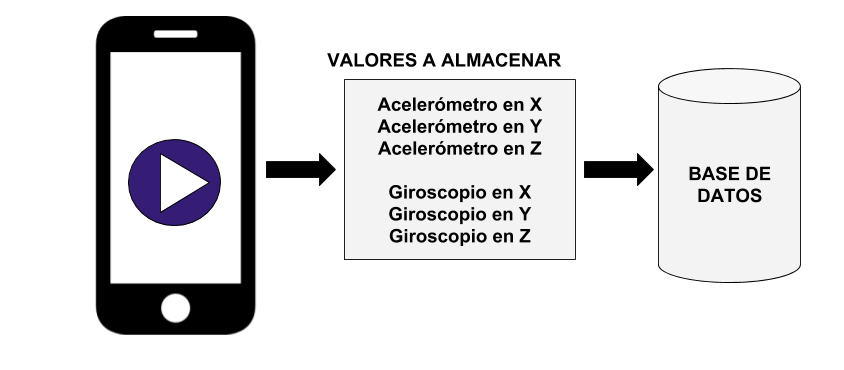
\includegraphics[width=0.95\textwidth,frame]{imagenes/Cap3/captura}
  \caption{Recolecci\'{o}n de datos, con intervalo de un segundo.}
  \label{fig:captura}
  \end{center}
\end{figure}

\vspace{5mm} %5mm vertical space

Para la captura de datos se us\'{o} un soporte para celular de parabrisas como se ve en la Figura \ref{fig:soporte}; se realiz\'{o} la captura en dos posiciones distintas (vertical y horizontal).
\vspace{5mm} %5mm vertical space

\begin{figure}[h!]
  \begin{center}	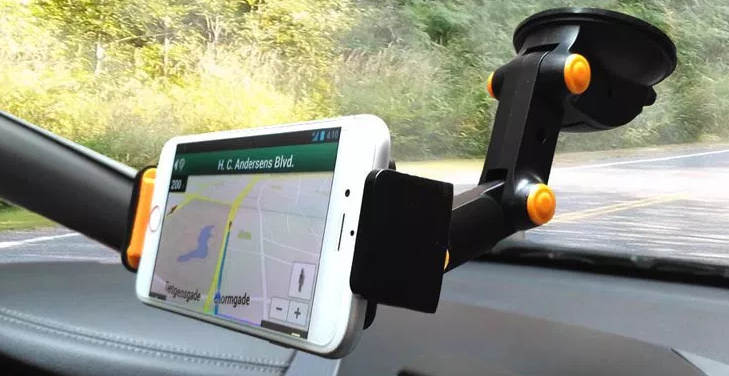
\includegraphics[width=0.65\textwidth,frame]{imagenes/Cap3/soporte}
  \caption{Soporte para celular de parabrisas, posici\'{o}n horizontal.}
  \label{fig:soporte}
  \end{center}
\end{figure}

Cada captura, independientemente de la posici\'{o}n en la que se realiz\'{o}, di\'{o} como resultado un conjunto de datos (dataset), donde por cada tiempo T (1 seg.) se tiene seis variables: aceler\'{o}metro en X (acc x), aceler\'{o}metro en Y (acc y), aceler\'{o}metro en Z (acc z), giroscopio en X (gyr x), giroscopio en Y (gyr y) y giroscopio en Z (gyr z). En la Figura \ref{fig:dataset} se aprecia un fragmento del conjunto de datos que se obtuvo en una captura.

\begin{figure}[h!]
  \begin{center}	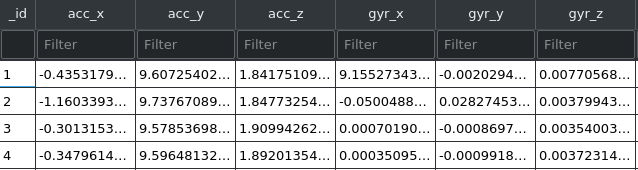
\includegraphics[width=0.95\textwidth,frame]{imagenes/Cap3/dataset}
  \caption{Fragmento del conjunto de datos obtenido.}
  \label{fig:dataset}
  \end{center}
\end{figure}

\section{Preparaci\'{o}n de datos}

El Aprendizaje Autom\'{a}tico depende en gran medida de los datos. Son el aspecto m\'{a}s crucial que hace posible el entrenamiento de algoritmos y explica porque el aprendizaje autom\'{a}tico se hizo tan popular en los \'{u}ltimos a\~{n}os. El principal problema es que todos los conjuntos de datos tienen fallas, lo que hace a la preparaci\'{o}n de datos un paso muy importante en el proceso de Aprendizaje Autom\'{a}tico.

\vspace{5mm} %5mm vertical space

El prop\'{o}sito principal de la preparaci\'{o}n de datos es manipular y transformar los datos en crudo, tal que, los datos puedan ser expuestos o hacerse accesibles m\'{a}s facilmente \cite{Reference37}, para lograr este prop\'{o}sito se debe seguir un proceso que implica la selecci\'{o}n, el pre-procesamiento y la transformaci\'{o}n de datos.
 
\subsection{Selecci\'{o}n de datos}

La selecci\'{o}n de datos implica los siguientes pasos:

\begin{itemize}
\item Seleccionar solo un subconjunto de los datos disponibles.
\item Derivar o simular algunos datos a partir de los datos diponibles, en caso de ser necesario.
\item Excluir aquellos datos que no son reelevantes para el problema.
\end{itemize}

Para el presente trabajo s\'{o}lo se har\'{a} incapi\'{e} en el primer paso de esta fase, debido a que los datos con los que se cuenta son limitados ya que \'{e}stos fueron capturados para la investigaci\'{o}n y como se indic\'{o} en la secci\'{o}n \ref{cap:CapDatos}, esta captura se realiz\'{o}, tanto de forma vertical como horizontal, a continuaci\'{o}n se analizar\'{a} las diferencias entre ellos.

\vspace{5mm} %5mm vertical space

En la Figura \ref{fig:verHor} se muestra fragmentos de las capturas obtenidas por el dispositivo m\'{o}vil de la conducci\'{o}n de un mismo usuario (agente) desde diferentes posiciones.

\begin{figure}
\fbox{
        \centering
        \begin{subfigure}[h]{0.47\textwidth} 
            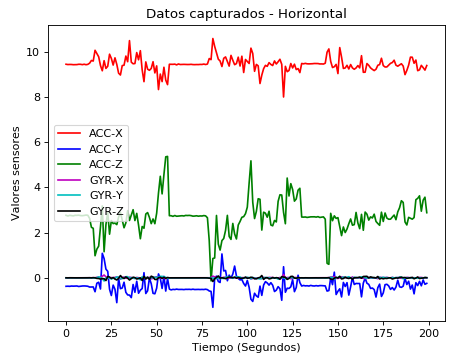
\includegraphics[width=\textwidth]{imagenes/Cap3/horizontal}
            \caption{Captura de datos en horizontal}
            \label{fig:hor}
        \end{subfigure}       
        \begin{subfigure}[h]{0.47\textwidth} 
            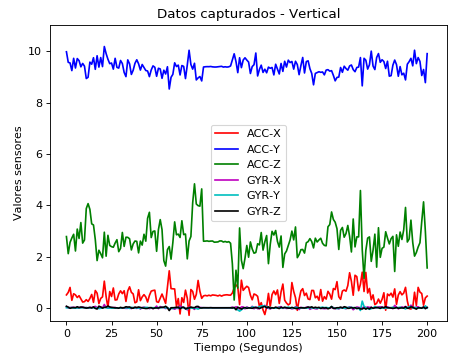
\includegraphics[width=\textwidth]{imagenes/Cap3/vertical}
            \caption{Captura de datos en vertical}
            \label{fig:ver}
        \end{subfigure}
        \caption{Gr\'{a}fica de los sensores capturados en diferentes posiciones.}
        		\label{fig:verHor}}
    \end{figure}

\vspace{5mm} %5mm vertical space

Si bien los valores capturados, son muy similares entre s\'{i}, los datos que fueron capturados con el dispositivo m\'{o}vil en posici\'{o}n horizontal, presentan menos ruido, esto debido a que esta posici\'{o}n favorece la inercia del dispositivo cuando el veh\'{i}culo est\'{a} en movimiento, lo cual es una gran ventaja frente a los datos que fueron capturados de forma vertical, ya que estos fueron m\'{a}s suceptibles a sacudirse mientras el veh\'{i}culo se desplazaba haciendo que los valores capturados en esta posici\'{o}n presenten valores de movimiento no s\'{o}lo del veh\'{i}culo sino tambi\'{e}n del dispositivo m\'{o}vil, lo cual no es lo que se busca en el presente trabajo.

\vspace{5mm} %5mm vertical space

Por las razones presentadas en el anterior p\'{a}rrafo se decidi\'{o} trabajar con los datos capturados con el dispositivo m\'{o}vil en posici\'{o}n horizontal, descartando as\'{i} aquellos datos capturados en vertical.

\section{Pre-procesamiento de datos}

Una vez que se seleccionaron los datos con los que se trabajar\'{a}, se debe proceder a pre-procesarlos, entrando as\'{i} a la fase de Pre-procesamiento de datos, el objetivo de esta fase es reducir la cantidad de los datos, encontrar las relaciones entre ellos, normalizarlos, remover los valores at\'{i}picos y extraer las caracter\'{i}sticas de los datos. Esta fase incluye varias t\'{e}cnicas como la limpieza, integraci\'{o}n, transformaci\'{o}n y reducci\'{o}n de los datos \cite{Reference38}.

\subsection{Limpieza de datos}

Los datos de las filas pueden tener registros incompletos, valores ruidosos, valores at\'{i}picos y datos inconsistentes. La limpieza de los datos en la mayor\'{i}a de los casos es el primer paso del pre-procesamiento de datos. Esta t\'{e}cnica se usa para compensar valores ausentes, suavizar el ruido en los datos, reconocer valores at\'{i}picos y corregir inconsistencias.

\subsubsection{T\'{e}cnicas de compensaci\'{o}n de registros incompletos}

Muchos conjuntos de datos del mundo real pueden contener valores faltantes por distintas razones; lo cual puede afectar drásticamente la calidad del modelo de aprendizaje automático. 

A continuaci\'{o}n se presentan cuatro t\'{e}cnicas de compensaci\'{o}n para conjuntos de datos, con el objetivo de sobrellevar el problema de los valores ausentes.

\begin{itemize}
\item \textbf{Ignorar / Eliminar:} En algunos casos es mejor ignorar o eliminar la tupla que contiene valores faltantes en lugar de llenar esta. Generalmente esta t\'{e}cnica se practica en conjuntos de datos que son muy grandes, donde el eliminar algunos datos no afectar\'{a} la informaci\'{o}n que transmite nuestro conjunto de datos. Sin embargo cuando se trabaja con un conjunto de datos peque\~{n}o el eliminar las tuplas que contienen valores ausentes podr\'{i}a hacer perder informaci\'{o}n importante.

\item \textbf{Llenar manualmente los valores ausentes:} Otra opci\'{o}n tambi\'{e}n es completar los valores faltantes si se comprende la naturaleza de los mismos, esto generalmente se realiza en conjunto de datos peque\~{n}os, ya que en los conjuntos grandes \'{e}sta tarea requerir\'{i}a bastante tiempo.

\item \textbf{Llenar los valores ausentes con valores centrales (Media/Mediana):} Esta t\'{e}cnica es mucho mejor que las presentadas anteriormente. En esta t\'{e}cnica se inserta la media o la mediana del atributo respectivo a los valores faltantes. 

\item \textbf{Interpolaci\'{o}n:} Es una forma confiable, precisa y cient\'{i}fica de completar valores perdidos. Para usar esta t\'{e}cnica primero se debe desarrollar una relaci\'{o}n entre los atributos y luego se predice el valor mas probable y preciso para los lugares faltantes, esto se puede lograr mediante regresi\'{o}n, formulaci\'{o}n bayesiana e inducci\'{o}n por \'{a}rboles de decisi\'{o}n.

\end{itemize}

\subsubsection{Eliminar rudio (suavizado) de los datos}

Para comprender esta t\'{e}cnica primero se debe definir qu\'{e} es el ruido en los datos. El ruido en los datos es cualquier tipo de error aleatorio o variaci\'{o}n en los atributos medidos; por otra parte los valores at\'{i}picos presentes en los datos tambi\'{e}n pueden considerarse como ruido. 

\vspace{5mm} %5mm vertical space

Es importante destacar que el ruido presente en el conjunto de datos puede afectar en gran medida el resultado de nuestros algoritmos de Aprendizaje Autom\'{a}tico, por lo tanto aquellos datos que contengan ruido no son considerados buenos datos y deben ser eliminados en lo posible. Sin embargo antes de eliminar estos, se debe ser capaz de detectarlos; para lograr este objetivo existen muchas t\'{e}cnicas que se pueden utilizar, una de estas t\'{e}cnicas es la \textbf{Visualizaci\'{o}n de datos}, la cual consiste en obtener una representaci\'{o}n visual de nuestros datos, para poder evidenciar si existe ruido en los datos y/o valores at\'{i}picos.

\vspace{5mm} %5mm vertical space

En el presente proyecto se grafic\'{o} histogramas de las frecuencias de cada caracter\'{i}stica de nuestro conjunto de datos y as\'{i} visualizar de mejor manera si existe ruido o valores at\'{i}picos en el mismo. En la Figura \ref{fig:hist} se puede evidenciar que los valores de cada sensor presentan asimetr\'{i}as negativas y positivas, adem\'{a}s de tener muchos valores bastante alejados de la media, lo que d\'{a} un indicio de posibles valores at\'{i}picos.

\begin{figure}[h!]
  \begin{center}	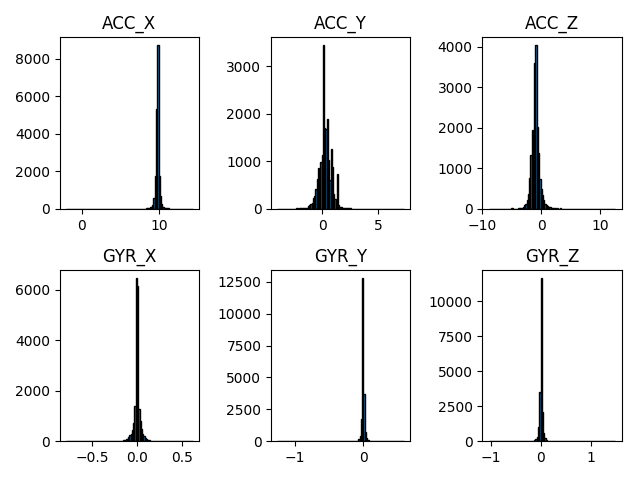
\includegraphics[width=0.97\textwidth,frame]{imagenes/Cap3/histograma_sensores}
  \caption{Histograma de frecuencias del conjunto de datos}
  \label{fig:hist}
  \end{center}
\end{figure}

\vspace{5mm} %5mm vertical space

En la Figura \ref{tab: est} se presenta una tabla con estad\'{i}sticas descriptivas de nuestro conjunto de datos, esta tabla presenta: la cantidad de datos, su media, su desviaci\'{o}n est\'{a}ndar, el valor m\'{i}nimo y m\'{a}ximo del conjunto de datos y los percentiles 50, 25 y 75, cabe recalcar que el percentil 50 es el mismo que la mediana.

\begin{figure}[h!]
  \begin{center}	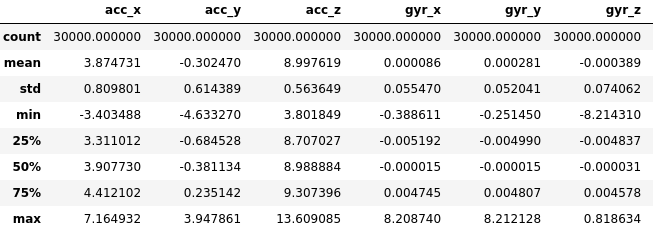
\includegraphics[width=0.97\textwidth,frame]{imagenes/Cap3/describe_data}
  \caption{Tabla de resultados estad\'{i}sticos del conjunto de datos.}
  \label{tab: est}
  \end{center}
\end{figure}

\vspace{5mm} %5mm vertical space

Con la informaci\'{o}n proporcionada en la Figura \ref{tab: est} ahora es m\'{a}s sencillo realizar un an\'{a}lisis del conjunto de datos, en primer lugar se evidencia que los valores obtenidos durante la captura, presentan desviaciones est\'{a}ndar muy peque\~{n}as entre 0.05 y 0.81 y sin embargo la diferencia entre los valores m\'{i}nimo y m\'{a}ximo son realmente grandes, por ejemplo para el Aceler\'{o}metro en X, la diferencia es 10 aproximadamente (Valor m\'{i}nimo: -3.40 y valor m\'{a}ximo: 7.17), esto quiere decir que nuestro conjunto de datos presenta mucho ruido, considerando como ruido o valores at\'{i}picos, aquellos valores muy alejados de la media. 

\vspace{5mm} %5mm vertical space

Para eliminar el ruido que presenta nuestro conjunto de datos se aplic\'{o} la \textbf{Regla 68-95-99.7}, conocida tambi\'{e}n como la \textbf{Regla emp\'{i}rica}, donde suponiendo que el conjunto de datos con el que se trabaja tiene una distribuci\'{o}n normal, la desviaci\'{o}n est\'{a}ndar se puede usar para determinar la proporci\'{o}n de valores que se encuentran dentro de un rango particular del valor medio. Para tales distribuciones, siempre ocurre que el 68\% de los valores est\'{a}n a menos de una desviaci\'{o}n est\'{a}ndar (1SD) del valor medio, que el 95\% de los valores est\'{a}n a menos de dos desviaciones est\'{a}ndar (2SD) de la media y que el 99\% de valores est\'{a}n a menos de tres desviaciones est\'{a}ndar (3SD) de la media. En la Figura \ref{fig:689599rule} se muestra este concepto de forma esquem\'{a}tica.

\begin{figure}[h!]
  \begin{center}	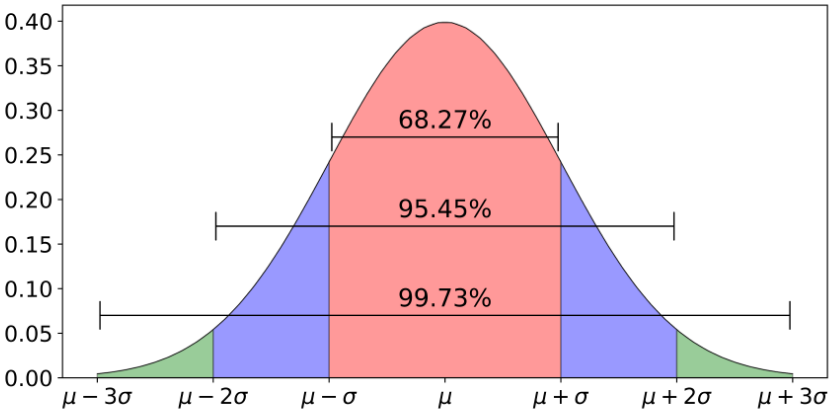
\includegraphics[width=0.97\textwidth,frame]{imagenes/Cap3/68-95-99_rule}
  \caption{Regla 68-95-99.7 }
  \label{fig:689599rule}
  \end{center}
\end{figure}

En la Figura \ref{fig:689599rule_acc_z}, se puede observar como se comporta la regla 68-95-99.7 sobre los valores del sensor del aceler\'{o}metro en Z, por lo que para eliminar el ruido en nuestro conjunto de datos se tiene dos opciones, eliminar los valores despu\'{e}s de tres desviaciones est\'{a}ndar de la media, en caso de considerar que nuestro conjunto de datos presenta pocas anomal\'{i}as o valores at\'{i}picos, o eliminar los valores despu\'{e}s de dos desviaciones est\'{a}ndar en caso de estar seguro que nuestro conjunto de datos presenta una gran cantidad de ruido en los datos, en nuestro caso la mayor\'{i}a de nuestros datos pertenecen a comportamientos normales de conducci\'{o}n por lo que s\'{o}lo se eliminar\'{a} los valores que se encuentran despu\'{e}s de tres desviaciones est\'{a}ndar de la media.


\begin{figure}[h!]
  \begin{center}	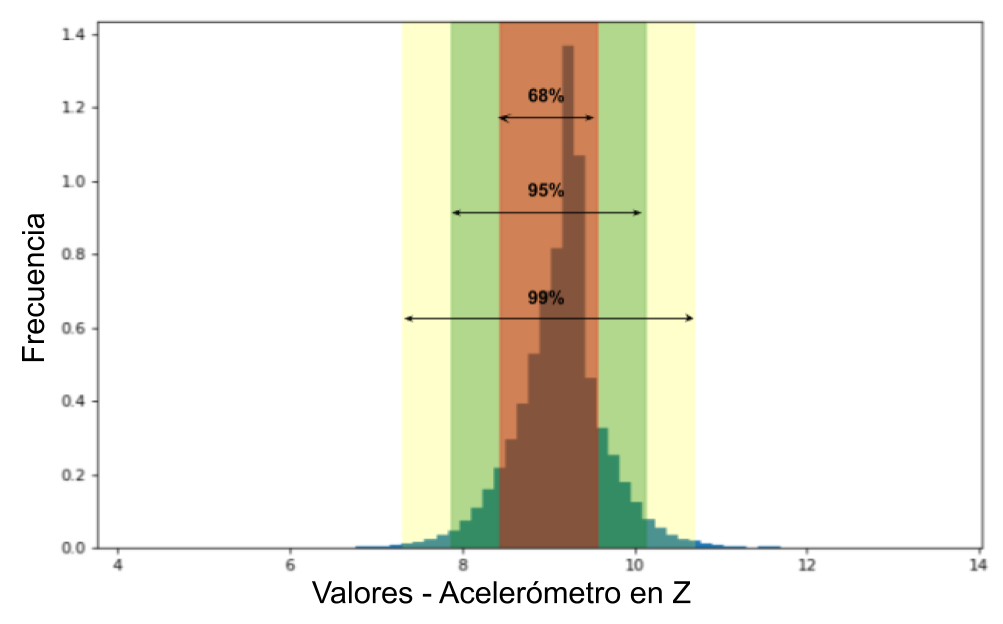
\includegraphics[width=0.97\textwidth,frame]{imagenes/Cap3/68-95-99_rule_acc_z}
  \caption{Regla 68-95-99.7 aplicada a los valores de los sensores del aceler\'{o}metro en Z. }
  \label{fig:689599rule_acc_z}
  \end{center}
\end{figure}

\subsubsection{Fusi\'{o}n o integraci\'{o}n de datos}

Cuando se trabaja con datos del mundo real, es posible que los datos que se requiere no se encuentren en un mismo conjunto de datos, en \'{e}stos casos, se necesita recopilar datos de diferentes fuentes y fusionarlos en un solo conjunto de datos; este proceso recibe el nombre de Fusi\'{o}n o Integraci\'{o}n de datos. Uno de los problemas m\'{a}s comunes de este proceso es la redundancia. 

\vspace{5mm} %5mm vertical space

Este proceso no se aplic\'{o} en la investigaci\'{o}n debido a que s\'{o}lo se captur\'{o} los datos por medio del dispositivo m\'{o}vil, por lo cual no se tiene el problema de tener m\'{a}s de una fuente de datos.

\subsubsection{Transformaci\'{o}n de datos}
\label{subsubsection:est-norm-dataset}

La transformaci\'{o}n de los datos es el proceso donde se cambia la naturaleza de los datos, dicho proceso usa algunas estrategias para poder extraer informaci\'{o}n importante del conjunto de datos; algunas de las estrategias para la transformaci\'{o}n de datos son: 

\begin{itemize}
\item \textbf{Agregaci\'{o}n: }En esta t\'{e}cnica, la operaci\'{o}n de resumen o agregaci\'{o}n se aplica sobre los datos. Por ejemplo: los datos de ventas diarias se pueden usar para calcular el monto mensual y anual en ventas, para posteriormente agregar estos datos calculados al conjunto de datos.

\item \textbf{Discretizaci\'{o}n: }Con esta t\'{e}cnica se construye y reemplaza valores en bruto de un atributo num\'{e}rico por valores de intervalo.

\item \textbf{Construcci\'{o}n de atributos / Ingenier\'{i}a de caracter\'{i}sticas: }Esta t\'{e}cnica es \'{u}til para generar informaci\'{o}n adicional a partir de aquellos datos que no son lo sufientemente representativos por s\'{i} mismos, adem\'{a}s puede ser adecuada cuando se tiene menos caracter\'{i}sticas pero a\'{u}n contienen informaci\'{o}n oculta para extraer.

\item \textbf{Normalizaci\'{o}n / Estandarizaci\'{o}n: }La normalizaci\'{o}n o estandarizaci\'{o}n se define como el proceso de reescalar datos originales sin cambiar su comportamiento o naturaleza. Se define un nuevo l\'{i}mite (generalmente entre 0 y 1) y se convierte los datos en consecuencia. Esta t\'{e}cnica es \'{u}til en algoritmos de clasificaci\'{o}n que involucran redes neuronales o algoritmos basados en la distancia (por ejemplo, KNN\footnote{\textbf{KNN}, es un algoritmo de clasificaci\'{o}n (o regresi\'{o}n) que, para determinar la clasificaci\'{o}n de un punto, combina la clasificaci\'{o}n de los $K$ puntos m\'{a}s cercanos.}, K-Means\footnote{\textbf{K-Means}, es un algoritmo de agrupamiento que intenta dividir un conjunto de puntos en $K$ grupos; de modo que los puntos en cada grupo tienden a estar cerca uno del otro.}, que se utiliza para la agrupaci\'{o}n. Este algoritmo es capaz de aprender gradualmente c\'{o}mo agrupar valores no etiquetados en grupos mediante un an\'{a}lisis de la distancia media de dichos valores.). Algunas t\'{e}cnicas de normalizaci\'{o}n son:
\begin{itemize}
\item \textit{Normalizaci\'{o}n Min-Max: }En este m\'{e}todo, cada entrada se normaliza entre unos l\'{i}mites definidos:

\begin{equation}
x_{normalizado} = \frac{x - x_{min}}{x_{max}-x_{min}}
\end{equation}

Presenta el problema de que comprime los datos de entrada entre unos límites fijos, que por lo general son 0 y 1. Esto quiere decir que si existe ruido, éste va a ser ampliado, lo que hace que este m\'{e}todo no sea adecuado para señales estables.

\item \textit{Escalado est\'{a}ndar (Standard Scaler): }Es un m\'{e}todo alternativo al escalado de variables, consiste en restar a cada dato la media de la variable y dividirlo por la desviaci\'{o}n t\'{i}pica.

\begin{equation}
x_{normalizado} = \frac{x - x_{media}}{x_{desvSt}}
\end{equation}

\'{E}ste m\'{e}todo es adecuado para normalizar se\~{n}ales estables, no obstante, tanto la media como la desviaci\'{o}n est\'{a}ndar son muy sensibles a valores an\'{o}malos. Una alternativa de soluci\'{o}n de \'{e}sto, es la eliminaci\'{o}n de anomal\'{i}as antes de realizar la normalizaci\'{o}n.

\item \textit{Escalado sobre el valor m\'{a}ximo: }Este m\'{e}todo, presenta la idea de escalar los datos dividiendo \'{e}stos entre su m\'{a}ximo valor.

\item \textit{Escalado robusto (Robust scaler): }El escalado robusto consiste en eliminar la mediana y escala los datos de acuerdo con el rango de interquartil (IQR). Este m\'{e}todo es robusto para valores at\'{i}picos.

\end{itemize}

\end{itemize}

\subsubsection{Reducci\'{o}n de datos}

Este proceso se basa en la adopci\'{o}n de algunas estrategias, tal que, el an\'{a}lisis de datos reducidos produce la misma informaci\'{o}n producida por los datos originales. Algunas de las estrategias incluyen: an\'{a}lisis de componentes principales (PCA), selecci\'{o}n de un subconjunto de atributos, agrupaci\'{o}n y muestreo entre otros.

\vspace{5mm} %5mm vertical space

\textbf{An\'{a}lisis de componentes principales (PCA)}

\vspace{5mm} %5mm vertical space

El An\'{a}lisis de Componentes Principales (PCA - Principal Component Analysis) es una técnica que se usa ampliamente para aplicaciones como reducción de dimensionalidad, compresión de datos con pérdida, extracción de características y visualización de datos \cite{Reference39}.

\vspace{5mm} %5mm vertical space

PCA es una t\'{e}cnica estad\'{i}stica no supervisada y no param\'{e}trica, que se utiliza para la reducci\'{o}n de dimensionalidad. Esta t\'{e}cnica es un paso importante debido a que la alta dimensionalidad en el campo de aprendizaje autom\'{a}tico puede llevar al sobreajuste del modelo, reduciendo as\'{i} su capacidad de generalizaci\'{o}n, \citeA{Reference40} describe este fen\'{o}meno como la "Maldici\'{o}n de la Dimensionalidad". Adem\'{a}s, el uso de esta t\'{e}cnica puede mejorar directamente el rendimiento de los modelos de Aprendizaje Autom\'{a}tico.

\vspace{5mm} %5mm vertical space

PCA combina las variables de entrada de una manera espec\'{i}fica, luego se deshace de las variables ''menos importantes'' y al mismo tiempo conserva las partes m\'{a}s valiosas (o componentes principales\footnote{\textbf{Componente principal}, es una combinaci\'{o}n lineal normalizada de las caracter\'{i}sticas originales en el conjunto de datos.}) de todas las variables.

\vspace{5mm} %5mm vertical space

Cuando se usa PCA enfocado al aprendizaje autom\'{a}tico se sigue los siguientes pasos:

\begin{enumerate}

\item Dividir el conjunto de datos \textit{d}-dimensional en conjunto de entrenamiendo, desarrollo y prueba.
\item Estandarizar / Normalizar el conjunto de datos seg\'{u}n el conjunto de entrenamiento.
\item Construir la matriz de covarianza.
\item Descomponer la matriz de covarianza en sus vectores y valores propios.
\item Ordenar los valores propios disminuyendo el orden para clasificar los vectores propios correspondientes.
\item Seleccionar \textit{k} vectores propios que corresponden a los \textit{k} valores propios m\'{a}s grandes, donde \textit{k} es la dimensionalidad del nuevo subespacio de entidad (\textit{k}<=\textit{d}).
\item Construir una matriz de proyecci\'{o}n \textbf{W} a partir de los "top" \textit{k} vectores propios.
\item Transformar el conjunto de entrenamiento de entrada \textit{d}-dimensional \textbf{X} utilizando la matriz de proyecci\'{o}n \textbf{W} para obtener el nuevo subespacio de caracter\'{i}stica \textit{k}-dimensional.

\end{enumerate}

\vspace{5mm} %5mm vertical space

\textbf{\textit{Divisi\'{o}n del conjunto de datos}}

\vspace{5mm} %5mm vertical space

Dado que se cuenta con un conjunto de datos para generar el modelo de Aprendizaje Autom\'{a}tico, este se divide en tres partes: conjunto de entrenamiento\footnote{\textbf{Conjunto de entrenamiento}, es la muestra de datos utilizada para ajustar el modelo de Aprendizaje Autom\'{a}tico.}, desarrollo\footnote{\textbf{Conjunto de desarrollo}, es la muestra de datos utilizada para proporcionar una evaluaci\'{o}n imparcial de un modelo ajustado con el conjunto de entrenamiento mientras se ajustan los hiperpar\'{a}metros del modelo.} y prueba\footnote{\textbf{Conjunto de prueba}, es la muestra de datos utilizada para proporcionar una evaluaci\'{o}n imparcial de un ajuste final del modelo en el conjunto de entrenamiento.}, sin embargo esto no es una tarea trivial; ya que si no se hace correctamente el resultado puede ser desastroso.

\vspace{5mm} %5mm vertical space

\begin{figure}[h!]
  \begin{center}	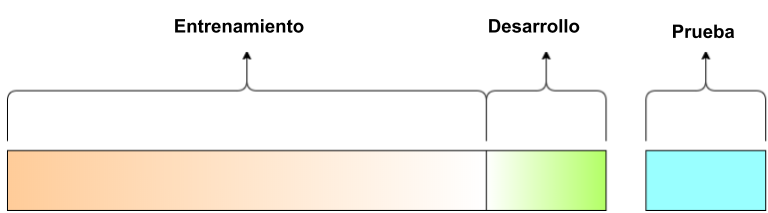
\includegraphics[width=0.97\textwidth,frame]{imagenes/Cap3/train-dev-test}
  \caption{Divisi\'{o}n del conjunto de entrenamiento.}
  \label{fig:train-dev-test}
  \end{center}
\end{figure}

En el trabajo de \citeA{Reference41} se dice que la divisi\'{o}n del conjunto de datos tiene un gran impacto en la productividad , por lo cual es importante que al elegir todos nuestros subconjuntos estos deben tener la \textbf{misma distribuci\'{o}n} y deben ser elegidos aleatoriamente del conjunto de datos. 

\vspace{5mm} %5mm vertical space

Por otra parte el tama\~{n}o del conjunto de desarrollo y prueba deben ser lo suficientemente grandes como para que los resultados del desarrollo y prueba sean representativos para el rendimiento del modelo. Para conjuntos de datos grandes (mayores a un mill\'{o}n), el conjunto de desarrollo y prueba puede tener alrededor de 10000 ejemplos cada uno, es decir, el 1\% del total de datos.

\vspace{5mm} %5mm vertical space

Otras consideraciones que deben tomarse en cuenta en la pr\'{a}ctica son:

\begin{itemize}
\item La divisi\'{o}n del conjunto de entrenamiento/desarrollo/prueba siempre debe ser la misma para todos los experimentos, por lo tanto se debe contar con script reproducible para crear la divisi\'{o}n entrenamiento/desarrollo/prueba.
\item Se debe probar que los conjuntos de desarrollo y prueba provengan de la misma distribuci\'{o}n.
\end{itemize}

En la presente investigaci\'{o}n nuestro conjunto de datos cuenta con 30000 ejemplos, por lo que la divisi\'{o}n de nuestro conjunto de datos ser\'{a} la que se observa en el Cuadro \ref{table:division-dataset}.


\begin{table}[]
\centering
\begin{tabular}{|l|l|l|}
\hline
Conjunto de entrenamiento & 70\%  & 21000 \\ \hline
Conjunto de desarrollo    & 15\%  & 4500  \\ \hline
Conjunto de prueba        & 15\%  & 4500  \\ \hline
Conjunto de datos         & 100\% & 30000 \\ \hline
\end{tabular}
\caption{Tabla de divisi\'{o}n del conjunto de datos.}
\label{table:division-dataset}
\end{table}

\vspace{5mm} %5mm vertical space

\textbf{\textit{Estandarizar / Normalizar el conjunto de datos}}

\vspace{5mm} %5mm vertical space

En la secci\'{o}n \ref{subsubsection:est-norm-dataset} ya se describi\'{o} lo que es la estandarizaci\'{o}n o normalizaci\'{o}n de datos y algunos de los tipos de escalado que existen; por lo tanto esta secci\'{o}n s\'{o}lo se limitar\'{a} a la elaboraci\'{o}n de un an\'{a}lisis para decidir que t\'{e}cnica de escalado es la m\'{a}s adecuada para el conjunto de datos, en la Figura \ref{fig:datos_puros} se puede apreciar una fracci\'{o}n del conjunto de datos capturado, la cual es la base con la que se realizar\'{a} el an\'{a}lisis comparativo con los distintos tipos de escalado.

\begin{figure}[h!]
  \begin{center}	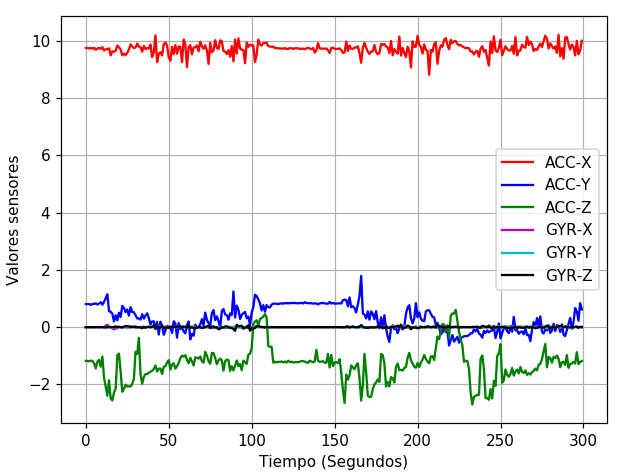
\includegraphics[width=0.5\textwidth,frame]{imagenes/Cap3/datos_sin_preprocesamiento}
  \caption{Visualizaci\'{o}n de los par\'{a}metros de conducci\'{o}n capturados.}
  \label{fig:datos_puros}
  \end{center}
\end{figure}

\vspace{5mm} %5mm vertical space

Para probar los diferentes tipos de escalado, se los ajusto con los datos que ya no presentan ruido o valores at\'{i}picos del conjunto de entrenamiento.

\begin{figure}
        \centering
        \fbox{\begin{varwidth}{\textwidth}
        \begin{subfigure}[h]{0.45\textwidth} 
            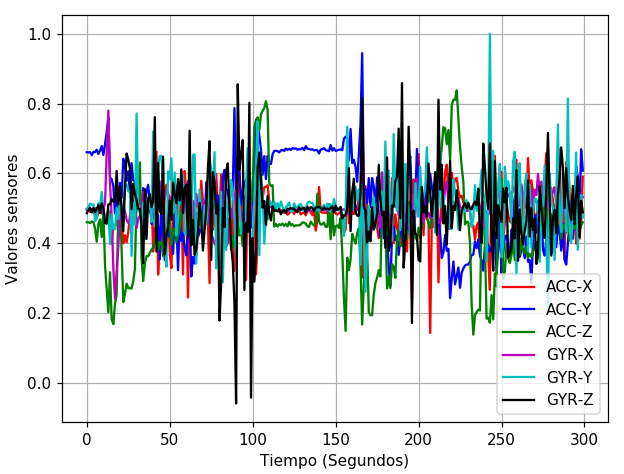
\includegraphics[width=\textwidth]{imagenes/Cap3/datos_minmax_scaler}
            \caption{Min max Scaler}
            \label{fig:min_max}
        \end{subfigure}       
        \begin{subfigure}[h]{0.45\textwidth} 
            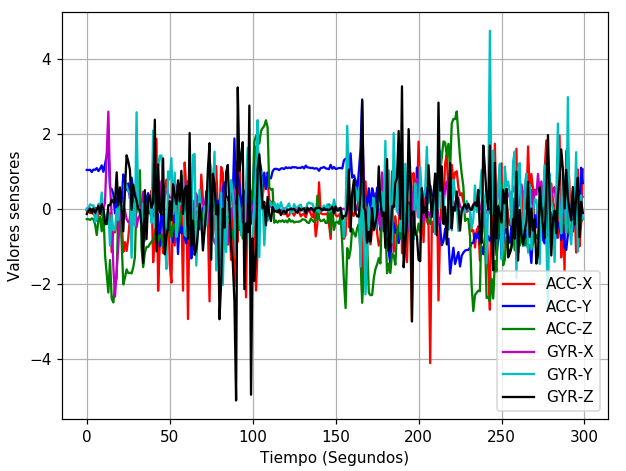
\includegraphics[width=\textwidth]{imagenes/Cap3/datos_standard_scaler}
            \caption{Standard Scaler}
            \label{fig:standard}
        \end{subfigure}
        
        \begin{subfigure}[h]{0.45\textwidth} 
            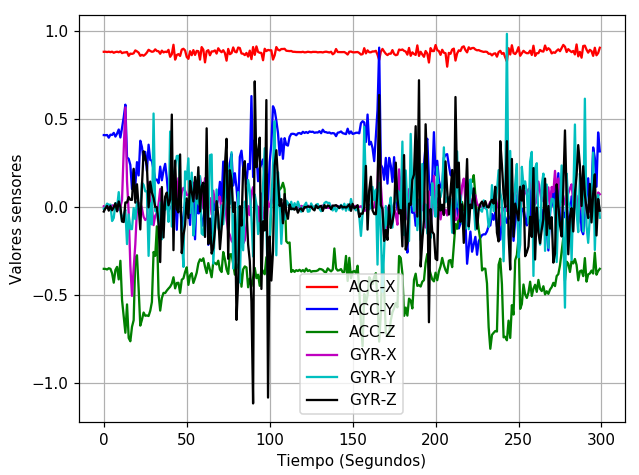
\includegraphics[width=\textwidth]{imagenes/Cap3/datos_max_scaler}
            \caption{Max Scaler}
            \label{fig:max}
        \end{subfigure}       
        \begin{subfigure}[h]{0.45\textwidth} 
            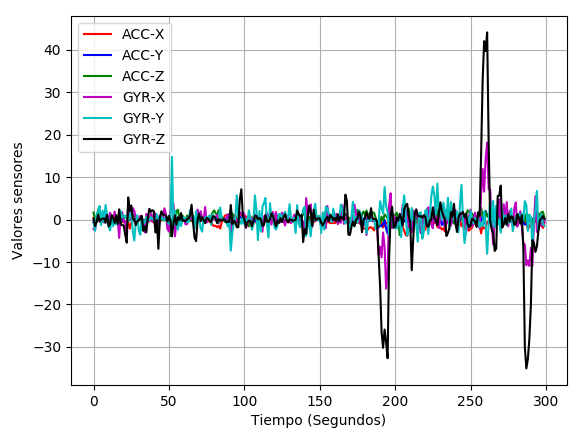
\includegraphics[width=\textwidth]{imagenes/Cap3/datos_robust_scaler}
            \caption{Robust Scaler}
            \label{fig:robust}
        \end{subfigure}
        \end{varwidth}}
        \caption{Gr\'{a}fica resultante de aplicar diferentes tipos de normalizaciones a un conjunto de datos.}
        
		\label{fig:nor_nor}
    \end{figure}

\vspace{5mm} %5mm vertical space

El primer tipo de escalado que se realiz\'{o} sobre el conjunto de datos capturados fue la \textbf{Normalizaci\'{o}n Min-Max}, el cual se realiz\'{o} entre los l\'{i}mites 0 y 1, los resultados obtenidos se muestran en la figura \ref{fig:min_max}, donde se puede apreciar que los valores del aceler\'{o}metro, en sus tres ejes, no se veen deformados despu\'{e}s de haber sido escalados con \'{e}sta t\'{e}cnica y los valores del giroscopio, los cuales son m\'{a}s estables se tornan deformados, considerando como datos estables aquellos datos que se presentan como una l\'{i}nea en cero con pocas fluctuaciones; esta deformaci\'{o}n puede ser ventajosa al hacer m\'{a}s visible peque\~{n}as curvas que anteriormente eran imperceptibles, sin embargo conlleva el peligro de que pueda ampliar ruido existente en nuestros datos que no pudimos eliminar en el paso previo a esta tarea.


\vspace{5mm} %5mm vertical space

La segunda t\'{e}cnica de normalizaci\'{o}n que se aplic\'{o} sobre los datos fue el \textbf{escalado est\'{a}ndar}, el resultado se puede apreciar en la figura \ref{fig:standard}, observando detalladamente los resultados se puede evidenciar que son muy similares a los obtenidos con la normalizaci\'{o}n Min-Max, las \'{u}nicas diferencias que se pueden evidenciar son que el nuevo rango de los datos es m\'{a}s amplio con media en cero y valores que oscilan principalmente entre 2 y -2,  y que se amplia un poco m\'{a}s algunas de las fluctuaciones que presentan los giroscopios.

\vspace{5mm} %5mm vertical space

Para la tercera normalizaci\'{o}n de datos se aplic\'{o} la t\'{e}cnica de \textbf{escalado sobre el valor m\'{a}ximo}, los resultados se presentan totalmente diferentes a los que se obtuvo anteriormente, sin embargo se observa claramente que los valores del aceler\'{o}metro no presentan mucho cambio, con la diferencia de que la media de estos valores son distintas para cada uno, y los valores de los giroscopios se comportan como en los anteriores, como se puede ver en la figura \ref{fig:max}. Esta t\'{e}cnica presenta los peores resultados, ya que no deja el conjunto de datos en un mismo rango lo cual complica el trabajo con dichos datos.

\vspace{5mm} %5mm vertical space

La \'{u}ltima t\'{e}cnica aplicada es el \textbf{escalado robusto}, su resultado puede ser observado en la figura \ref{fig:robust}, el cual puede ser considerado bastante similar a las dos primeras t\'{e}cnicas, con diferencia de que este escalado pronuncia mucho m\'{a}s las fluctuaciones de los valores de los giroscopios, convirti\'{e}ndolos incluso a una escala superior que el de los valores de los aceler\'{o}metros.

\vspace{5mm} %5mm vertical space

Para decidir el mejor m\'{e}todo de normalizaci\'{o}n que se puede aplicar a los datos capturados, primero se descartar\'{a} completamente el \textbf{m\'{e}todo de escalado sobre el valor m\'{a}ximo} debido a que los resultados que present\'{o} fueron totalmente desalentadores ya que los valores despu\'{e}s del escalado no compart\'{i}an los mismos l\'{i}mites, por otra parte los restantes tres tipos de escalado son muy similares, lo cual complica la elecci\'{o}n de escalado correcto, sin embargo cuando se usa PCA se debe ser muy cuidadoso, debido a que si se tiene una variable con una desviaci\'{o}n est\'{a}ndar alta, esta tendr\'{a} un mayor peso en el c\'{a}lculo del eje que una variable con una desviaci\'{o}n est\'{a}nda baja, por lo cual este puede ser un par\'{a}metro de decisi\'{o}n importante para elegir el tipo de escalado m\'{a}s adecuado.

\vspace{5mm} %5mm vertical space

En la tabla \ref{table:scalers} se muestra la media y la desviaci\'{o}n est\'{a}ndar de cada variable despu\'{e}s de haber aplicado los diferentes tipos de escalado sobre los datos. Como se puede evidenciar en los escalados sobre el valor m\'{a}ximo y est\'{a}ndar, las desviaciones est\'{a}ndar son muy diferentes, en cuanto al escalado Min-Max las desviaciones est\'{a}ndar de cada variable son casi las mismas ya que todas oscilan entre 0.166814 y 0.169386, lo cual se adec\'{u}a muy bien para el an\'{a}lisis de componentes principales, mencionando adem\'{a}s que esta t\'{e}cnica es la que mejor conserva la informaci\'{o}n relevante del conjunto de datos, por lo cual esta t\'{e}cnica fue la seleccionada debido a que es la m\'{a}s conveniente para esta etapa.

\begin{landscape}
\pagestyle{empty}
\begin{table}[p!]

\centering
\begin{tabular}{ll|r|r|r|r|r|r|}
\cline{3-8}
 &  & \multicolumn{1}{c|}{\textbf{ACC X}} & \multicolumn{1}{c|}{\textbf{ACC Y}} & \multicolumn{1}{c|}{\textbf{ACC Z}} & \multicolumn{1}{c|}{\textbf{GYR X}} & \multicolumn{1}{c|}{\textbf{GYR Y}} & \multicolumn{1}{c|}{\textbf{GYR Z}} \\ \hline
\multicolumn{1}{|l|}{\multirow{4}{*}{Min-Max}} & Media & 0.500369	 & 0.500051 & 0.501112 & 0.497923 & 0.499352 & 0.500396 \\ \cline{2-8} 
\multicolumn{1}{|l|}{}                  & Desv. Est. & 0.166847 & 0.166814 & 0.167300 & 0.168245 & 0.169386 & 0.166852 \\ \cline{2-8} 
\multicolumn{1}{|l|}{}                  & M\'{i}nimo & -0.999198 & -0.675814	& -1.041074 & -0.681029 & -0.319990 & -18.004503 \\ \cline{2-8} 
\multicolumn{1}{|l|}{}                  & M\'{a}ximo & 1.178265 & 1.654068 & 1.869867 & 25.395520 & 27.227514 & 2.345548 \\ \hline
\multicolumn{1}{|l|}{\multirow{4}{*}{Est\'{a}ndar}} & Media & -0.011266 & -0.009209 & -0.00570 & 0.013265 & 0.009458 & 0.005644 \\ \cline{2-8} 
\multicolumn{1}{|l|}{}                  & Desv. Est. & 1.050384 & 1.086118 & 1.117567 & 2.224617 & 2.518566 & 2.076506 \\ \cline{2-8} 
\multicolumn{1}{|l|}{}                  & M\'{i}nimo & -9.451768 & -7.665204 & -10.307538 & -15.575414	 & -12.173164 & -230.291158 \\ \cline{2-8} 
\multicolumn{1}{|l|}{}                  & M\'{a}ximo & 4.256420 & 7.504531 & 9.137616 & 329.221266 & 397.424938 & 22.968890 \\ \hline
\multicolumn{1}{|l|}{\multirow{4}{*}{Valor M\'{a}ximo}} & Media & 0.615065 & -0.141064 & 0.842598 & 0.000519 & 0.001827 & -0.001747 \\ \cline{2-8} 
\multicolumn{1}{|l|}{}                  & Desv. Est. & 0.128546 & 0.286536 & 0.052784 & 0.334925 & 0.337715 & 0.332858 \\ \cline{2-8} 
\multicolumn{1}{|l|}{}                  & M\'{i}nimo & -0.540261 & -2.160843	& 0.356031 & -2.346416 & -1.631746 & -36.917638 \\ \cline{2-8} 
\multicolumn{1}{|l|}{}                  & M\'{a}ximo & 1.137343 & 1.841185 & 1.274447 & 49.564032 & 53.291415 & 3.679194 \\ \hline
\multicolumn{1}{|l|}{\multirow{4}{*}{Robusto}} & Media & -0.028625 & 0.083278 & 0.008976 & 0.010491 & 0.031468 & -0.040602 \\ \cline{2-8} 
\multicolumn{1}{|l|}{}                  & Desv. Est. & 0.739033 & 0.672602 & 0.956915 & 5.752011 & 5.518751 & 8.397460 \\\cline{2-8} 
\multicolumn{1}{|l|}{}                  & M\'{i}nimo & -6.670812 & -4.657858	& -8.811955 & -40.295886 & -26.663430 & -931.368512 \\ \cline{2-8} 
\multicolumn{1}{|l|}{}                  & M\'{a}ximo & 2.974050 & 4.736319 & 7.837925 & 851.216772 & 870.859223 & 92.823529 \\ \hline
\end{tabular}
\caption{Tabla con estad\'{i}sticas descriptivas de los datos escalados con diferentes t\'{e}cnicas.}
\label{table:scalers}
\end{table}
\end{landscape}


\pagestyle{thesis}

\vspace{5mm} %5mm vertical space

\textbf{\textit{Aplicar PCA al conjunto de datos}}

\vspace{5mm} %5mm vertical space

Aunque al inicio de esta subsubsecci\'{o}n se explica en detalle algunos de los pasos del funcionamiento interno de PCA, existe una clase llamada PCA implementada en \textsc{scikit-learn}, la cual automatiza todos los pasos siguientes; sin embargo se necesita determinar cu\'{a}ntas caracter\'{i}sticas (componentes principales) mantener y cu\'{a}ntas eliminar; para \'{e}sta tarea existen tres m\'{e}todos com\'{u}nmente utilizados, los cuales ser\'{a}n descritos a continuaci\'{o}n.

% https://towardsdatascience.com/a-one-stop-shop-for-principal-component-analysis-5582fb7e0a9c
\begin{itemize}
\item Seleccionar arbitrariamente cu\'{a}ntas dimensiones se desea mantener, dependiendo del caso de uso. Por ejemplo, para un enfoque de visualizaci\'{o}n se podr\'{i}a elegir 2 o 3 caracter\'{i}sticas.
\item Calcular la proporci\'{o}n de la varianza para cada caracter\'{i}stica, elegir un umbral y agregar  caracter\'{i}sticas hasta llegar o superar el umbral elegido.
\item Este m\'{e}todo est\'{a} estrechamente relacionado con el anterior, debido a que se calcula la proporci\'{o}n de varianza para cada caracter\'{i}stica, se ordena las caracter\'{i}sticas por la proporci\'{o}n de varianza y se traza la proporci\'{o}n de varianza acumulada explicada a medida que mantiene las caracter\'{i}sticas (este diagrama es conocido como \textit{diagrama de pantalla}). Se puede elegir cu\'{a}ntas caracter\'{i}sticas incluir al identificar el punto en el que se agrega una nueva caracter\'{i}stica tiene una ca\'{i}da significativa en la variaci\'{o}n en relaci\'{o}n con la caracter\'{i}stica anterior, y elegir la cantidad de caracter\'{i}sticas que existen hasta ese punto. Este m\'{e}todo suele ser conocido como \textit{''Encontrar el codo''}.
\end{itemize}

Para el desarrollo de la presente investigaci\'{o}n se descart\'{o} tanto el primer y \'{u}ltimo m\'{e}todo de los listados anteriormente, esto debido a que el primer m\'{e}todo no tiene la certeza de que la cantidad de caracter\'{i}sticas que se elige sea lo suficientemente descriptiva para el conjunto de datos; mientras que el \'{u}ltimo m\'{e}todo no cuenta con una definici\'{o}n matem\'{a}ticamente precisa, debido a que s\'{o}lo encuentra el ''codo'', por lo que tambi\'{e}n quita el control de la cantidad de variabilidad total en los datos que se obtiene finalmente.

\vspace{5mm} %5mm vertical space

Una vez descartados los m\'{e}todos que no se ajustan al requerimiento del presente trabajo, la \'{u}nica opci\'{o}n restante es el segundo m\'{e}todo, siendo as\'{i} este el que se aplicar\'{a} para el presente trabajo. Por lo tanto primero se defini\'{o} como 90\% el umbral de variabilidad total que se desea preservar en el conjunto de datos, posteriormente haciendo uso de la clase PCA de \textsc{scikit-learn} se calcula la varianza de cada caracter\'{i}stica y posteriormente se grafica los resultados (Ver Figura \ref{fig:varianza-pca}).

\begin{figure}[h!]
  \begin{center}	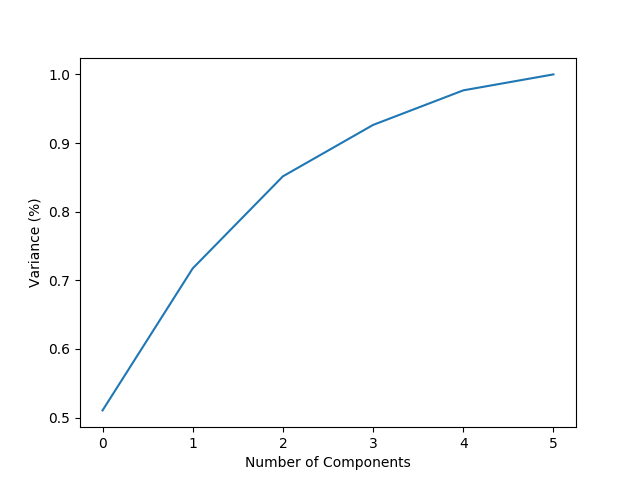
\includegraphics[width=0.75\textwidth,frame]{imagenes/Cap3/pca}
  \caption{Gr\'{a}fico de la varianza vs. el n\'{u}mero de componentes.}
  \label{fig:varianza-pca}
  \end{center}
\end{figure}

\vspace{5mm} %5mm vertical space

Y por \'{u}ltimo se debe definir que cantidad de componentes principales conservan el 90\% de la varianza de los datos como m\'{i}nimo. La Gr\'{a}fico \ref{fig:varianza-pca} indica que seleccionando 4 componentes se puede preservar alrededor del 97.7\% de la varianza total de los datos, seleccionando 3 componentes se conserva alrededor del 92.3\% y seleccionando 2 se conserva el 85\% de la varianza; por lo tanto se decidi\'{o} el uso de 3 caracter\'{i}sticas con lo cual se conservar\'{a} el 92.3\% de la varianza total del conjunto de datos.

\vspace{5mm} %5mm vertical space

En diversos estudios (\citeNP{Reference63}; \citeNP{Reference64}) se prob\'{o} que la aplicaci\'{o}n de PCA como pre-procesamiento del conjunto de datos es una etapa importante, debido a que no s\'{o}lo sirve para la compresi\'{o}n de los datos de entrada, sino que tambi\'{e}n proporciona una mejora satisfactoria de la precisi\'{o}n de los modelos de Aprendizaje Autom\'{a}tico; raz\'{o}n por la cual esta t\'{e}cnica forma parte de la etapa de pre-procesamiento de este trabajo.

\section{Resumen del cap\'{i}tulo}

En este cap\'{i}tulo se ha descrito la forma en la que se realiz\'{o} la captura del conjunto de datos de conducci\'{o}n y su preparaci\'{o}n, mediante distintas t\'{e}cnicas como la selecci\'{o}n, limpieza, reducci\'{o}n y transformaci\'{o}n de datos; con el fin de que estos valores sean una mejor entrada para el algoritmo de detecci\'{o}n de anomal\'{i}as que se detallar\'{a} en el siguiente cap\'{i}tulo.